\documentclass[a4paper,12pt]{report}

\usepackage{alltt, fancyvrb, url}
\usepackage{graphicx}
\usepackage[utf8]{inputenc}
\usepackage{float}
\usepackage{hyperref}

% Questo commentalo se vuoi scrivere in inglese.
\usepackage[italian]{babel}
\usepackage[italian]{cleveref}
\usepackage[margin=1in]{geometry}

% Set the top margin to 0.5 inch
\setlength{\topmargin}{-0.3in}

\setlength{\parindent}{0pt}

\title{\textbf{Elaborato per il corso di\\"Basi di Dati"}
\\A.A. 2023/24}

\author{Gioele Bucci
\\ \texttt{gioele.bucci@studio.unibo.it}}
\date{\today}


\begin{document}

\maketitle

\tableofcontents

\chapter{Analisi dei requisiti}

Si vuole realizzare un sistema che consenta agli utenti di poter salvare ed analizzare delle partite al gioco da tavolo di strategia “RisiKo!”.
Ogni partita va memorizzata nel database, includendo i singoli turni: per ciascun turno deve essere possibile visualizzare sia lo stato di gioco che le azioni eseguite dal giocatore di turno.

\section{Intervista}

Un primo testo ottenuto dall’intervista è il seguente: \\ \\
Si vuole sviluppare un sistema che consenta agli utenti di memorizzare delle partite di Risiko, permettendo di visualizzarne lo stato nei vari turni. Per ciascun utente vengono salvati codice fiscale, nome, cognome e data di nascita. Un utente può partecipare come giocatore a più partite. \par
Ogni partita è caratterizzata da un codice identificativo, la data nella quale è avvenuta e il giocatore vincitore.
Ad ogni partita possono partecipare da 3 a 6 giocatori: per ciascuno si vuole memorizzare il relativo utente, un nickname, il colore dell’esercito scelto e l’obiettivo personale. \par
L’area di gioco è composta da un insieme di territori, identificati univocamente da un nome e per cui si memorizzano anche la lista di territori confinanti e il continente di appartenenza. \par
All’inizio di una partita ciascun giocatore riceve un numero predeterminato di carri armati, che dipende dal numero totale di giocatori partecipanti. Tutti i territori vengono poi distribuiti equamente tra i giocatori in modo casuale. In seguito, ogni giocatore posiziona tutte le sue armate sui propri territori, occupandone ciascuno con almeno un’unità. \par
Durante una partita, i giocatori si alternano ciclicamente in turni. \par
All’inizio di ogni turno avviene la fase di rinforzo, nella quale il giocatore di turno riceve una nuova armata per ogni tre territori in suo possesso. In aggiunta, il possesso di tutti i territori di un continente conferisce un bonus di armate aggiuntivo, che dipende dal continente conquistato. \par 
Le nuove armate ottenute vanno immediatamente posizionate dal giocatore di turno su uno o più territori che gli appartengono.
Ciascun turno all’interno di una partita è identificato da un numero e il nome del giocatore di turno. In aggiunta vanno registrati anche il numero di truppe presenti sui territori del giocatore dopo la fase di rinforzo, ed eventuali azioni compiute (uno spostamento e/o un attacco). \par
Per poter attaccare un territorio avversario, l’attaccante deve controllare un territorio ad esso adiacente. Per ciascun attacco vanno memorizzati l’attaccante, il difensore, il numero di truppe impiegate e perse da entrambe le parti e l’eventuale successo dell’attacco, che è considerato riuscito se tutte le truppe sul territorio avversario vengono eliminate. \par
Lo spostamento consiste nel muovere una parte delle proprie truppe da un territorio ad un altro ad esso adiacente (entrambi i territori devono appartenere allo stesso giocatore). Per ciascuno spostamento vanno memorizzati il territorio di partenza, quello di arrivo e il numero di truppe mobilitate. \par
I territori non possono mai essere lasciati vuoti e tale vincolo vale anche nel caso di attacchi e spostamenti: in entrambi i casi occorre che nel territorio di partenza rimanga almeno un’unità. Questo implica che in ogni momento di gioco ciascun territorio è controllato da un giocatore.

\section{Estrazione dei concetti principali}

\begin{itemize}
    \item \textbf{Utente}: persona fisica iscritta al sistema. Può partecipare a più partite come giocatore.
    \item \textbf{Giocatore}: colui che partecipa ad una partita. Ogni giocatore è associato ad un utente ed ha un colore, che rappresenta il suo esercito nel gioco, e un singolo obiettivo.
    \item \textbf{Obiettivo}: traguardo che un giocatore deve raggiungere per vincere la partita.
    \item \textbf{Territorio}: specifica regione di gioco, controllata da un solo giocatore alla volta. Ha dei territori confinanti e fa parte di un continente.
    \item \textbf{Continente}: insieme di più territori. Il possesso di un continente da parte di un giocatore gli conferisce un bonus di armate aggiuntive all’inizio del turno.
    \item \textbf{Armata}: unità militare controllata da un giocatore, utilizzata per conquistare e difendere territori. \\\textit{Sinonimi: unità, carro armato, truppa.}
    \item \textbf{Turno}: fase della partita comprendente una serie di azioni compiute da un singolo giocatore. I turni si susseguono ciclicamente tra i vari giocatori fino al termine della partita.
    \item \textbf{Attacco}: azione che un giocatore può svolgere nel proprio turno. Durante un attacco, il giocatore utilizza le armate presenti in un suo territorio per tentare di conquistare un territorio avversario adiacente.
    \item \textbf{Spostamento}: azione che un giocatore può svolgere nel proprio turno. Consiste nel muovere una parte di armate da un suo territorio ad uno adiacente, anch’esso di sua proprietà.

\end{itemize}

A seguito della lettura e comprensione dei requisiti, si procede redigendo un testo che ne riassuma tutti i concetti e in particolare ne estragga quelli principali eliminando le ambiguità sopra rilevate: \\ \\
Per ogni \textbf{\textit{utente}} del sistema vengono memorizzati codice fiscale, nome, cognome e data di nascita. \par
Ogni \textbf{\textit{partita}} è associata ad un codice identificativo, una data e un vincitore. \par
Ad una partita possono partecipare da 3 a 6 \textbf{\textit{giocatori}}: per ciascuno si memorizzano il relativo utente, un nickname, il colore dell'esercito scelto e l’obiettivo personale. \par
L’area di gioco è composta da vari \textbf{\textit{territori}}, identificati dal nome, e di cui si memorizzano anche la lista di territori confinanti e il continente di appartenenza. In ogni momento di gioco ciascun territorio è controllato da un solo giocatore.
Il numero di \textbf{\textit{armate}} conferite ad ogni giocatore all’inizio della partita viene stabilito in base al numero totale dei giocatori partecipanti. \par
Durante la partita, i giocatori si alternano ciclicamente in turni. Ogni \textbf{\textit{turno}} è identificato univocamente all’interno di una partita da un numero e il nome del giocatore di turno. Vanno inoltre memorizzati il numero di truppe presenti su ciascuno dei territori del giocatore, dopo la fase di rinforzo, ed eventuali azioni compiute. \par
Nella fase di rinforzo, che avviene all’inizio del turno, il giocatore riceve una nuova armata per ogni tre territori posseduti, oltre ad un eventuale bonus aggiuntivo per ogni \textbf{\textit{continente}} posseduto: tale bonus dipende dal continente. \par
Durante il proprio turno un giocatore può effettuare un attacco ad un territorio avversario e/o uno spostamento tra due territori adiacenti di sua proprietà. \par
Per ogni \textbf{\textit{attacco}} si registrano l'attaccante, il difensore, il numero di armate impiegate e perse da entrambe le parti e l'esito dell'attacco, che è considerato riuscito se tutte le armate sul territorio attaccato vengono eliminate. \par
Per ogni \textbf{\textit{spostamento}} si vogliono memorizzare il numero di armate mobilitate, il territorio di partenza e quello di arrivo.

\chapter{Progettazione concettuale}

Dall'analisi del dominio emerge che un \textbf{utente }è associato ad una persona fisica (l'identificatore è infatti il codice fiscale), mentre l'esistenza dell'entità \textbf{giocatore }è circoscritta alla specifica \textbf{partita} a cui partecipa. \par
La partecipazione all'associazione \textbf{vincitore}, che collega una partita ad un giocatore, è resa opzionale al fine di rendere possibile salvare anche partite non concluse. Inoltre, al giocatore devono essere associati l'\textbf{esercito} scelto e l'\textbf{obiettivo}, resi tramite delle entità. 

\begin{figure}[H]
\centering{}
\begin{center}
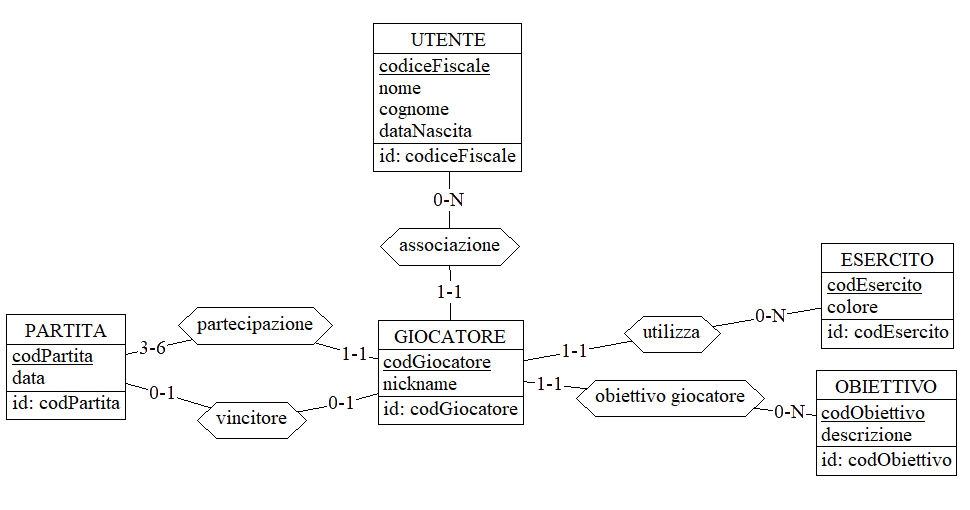
\includegraphics[width=\textwidth]{img/report/utente.png}
\end{center}
\emph{\caption{Schema E/R con le entità per la modellazione degli utenti e giocatori}}
\label{img:utente}
\end{figure}

Una partita è suddivisa in più turni: ciascun \textbf{turno} è identificato univocamente all'interno della partita mediante un numero e il nome del giocatore di turno. Pertanto, si utilizzano come identificatori il numero del turno, il giocatore (tramite l'associazione \textbf{effettuazione turno}) e la partita (tramite l'associazione \textbf{suddivisione}).   \par
Per memorizzare i \textbf{territori} posseduti e il numero di \textbf{armate} presenti su di essi, si utilizza l'associazione \textbf{controllo territorio}.

\begin{figure}[H]
\centering{}
\begin{center}
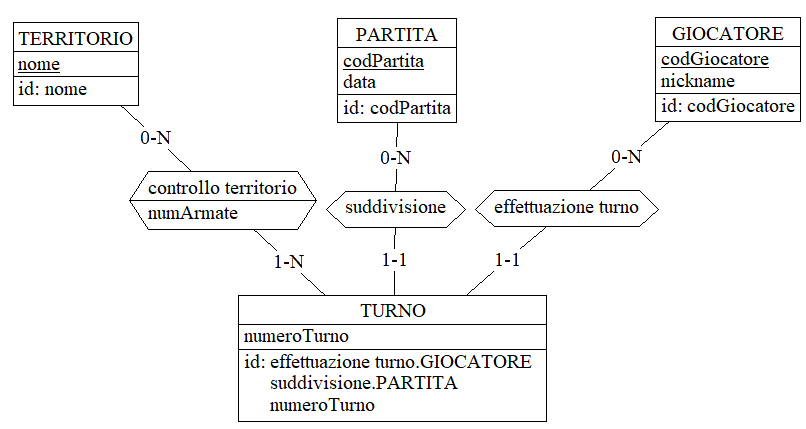
\includegraphics[width=\textwidth]{img/report/turno_par.png}
\end{center}
\emph{\caption{Schema E/R con una modellazione parziale dei turni}}
\label{img:turno_par}
\end{figure}
In ogni turno si possono effettuare un \textbf{attacco} e uno \textbf{spostamento}, entrambi resi tramite entità e identificati da un codice univoco. \par
L’esito di un attacco è dato dalla flag booleana \textit{vittoria}, mentre il territorio \textbf{attaccante} e quello \textbf{difensore} sono resi tramite associazioni. \par
Ci sono dei vincoli inespressi per cui il territorio attaccante e quello difensore devono essere diversi, confinanti e appartenenti a giocatori differenti. \par
Gli spostamenti sono modellati in maniera analoga agli attacchi e nell’entità si memorizza il numero di armate mobilitate. Il territorio di partenza e quello di arrivo sono resi, rispettivamente, dalle associazioni \textbf{da}, \textbf{a}. \par
Anche in questo caso ci sono dei vincoli inespressi per cui il territorio di partenza e quello di arrivo devono essere diversi, confinanti e appartenenti allo stesso giocatore. 

\begin{figure}[H]
\centering{}
\begin{center}
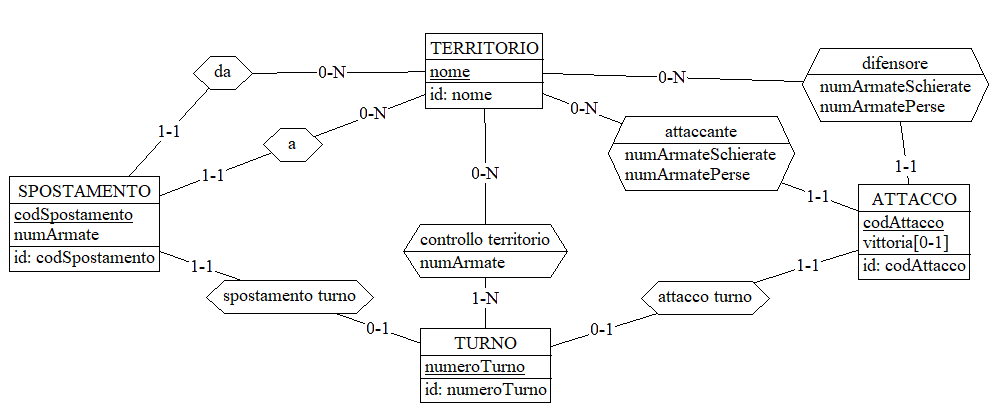
\includegraphics[width=\textwidth]{img/report/turno.png}
\end{center}
\emph{\caption{Schema E/R con la modellazione completa dei turni}}
\label{img:turno_par}
\end{figure}

Ogni territorio confina con almeno un’altro territorio (associazione ad anello simmetrica \textbf{confinante}) e fa parte di un \textbf{continente}, modellato tramite un’entità e identificato univocamente dal nome. \par
Infine, per memorizzare il numero di armate iniziali da assegnare in base al numero totale di giocatori, è stata aggiunta un’entità \textbf{armate iniziali}. \par
Di seguito lo schema finale:
\begin{figure}[H]
\centering{}
\begin{center}
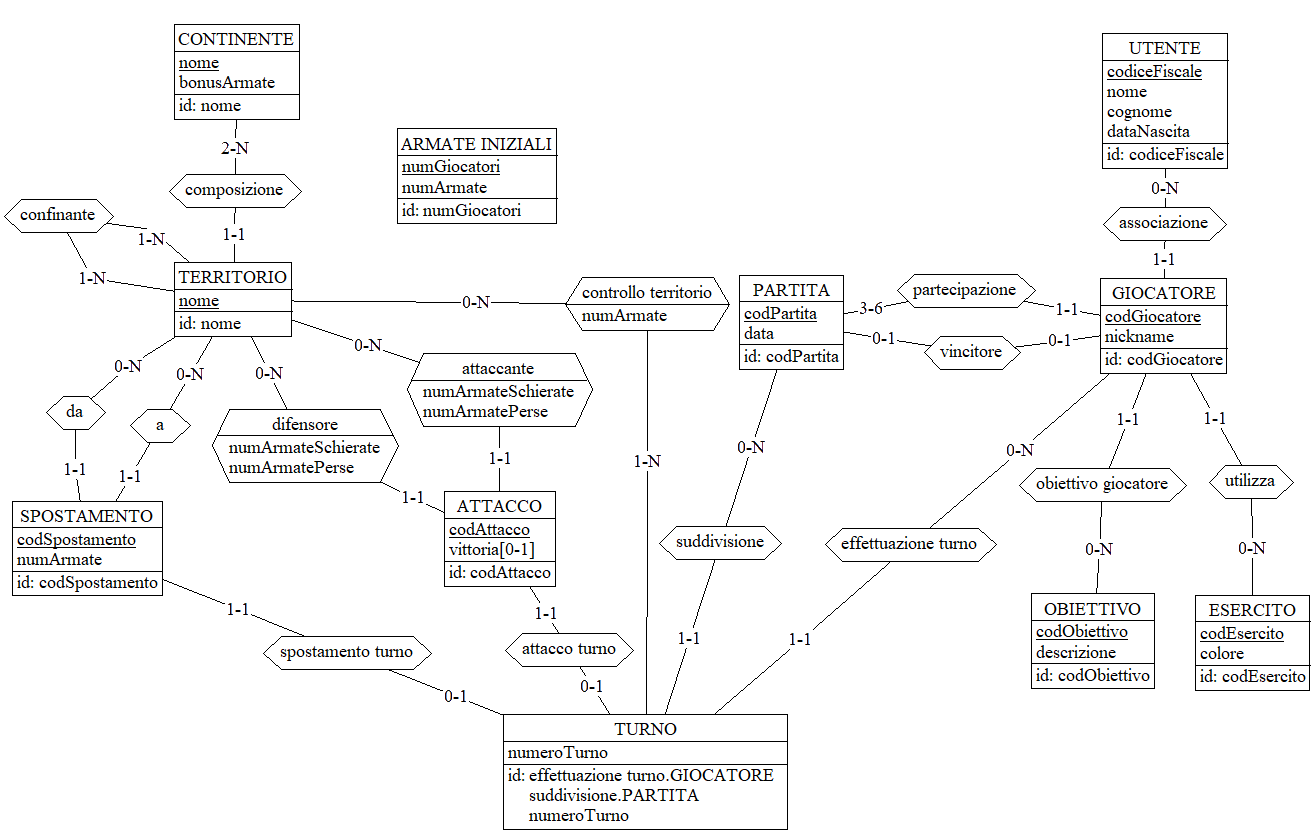
\includegraphics[width=\textwidth]{img/report/finale.png}
\end{center}
\label{img:turno_par}
\end{figure}

\chapter{Progettazione logica}
\section{Stima del volume dei dati}

\begin{table}[H]
    \caption{My Spreadsheet}
    \centering
    \begin{tabular}{|c|c|c|}
        \hline
        \textbf{Concetto}& \textbf{Costrutto}& \textbf{Volume}\\ \hline
        Continente & E & 6 \\ \hline 
        Composizione & A & 42 \\ \hline 
        Territorio & E & 42 \\ \hline 
        Confinante & A & 200 \\ \hline 
        Armate Iniziali & E & 4 \\ \hline
        Obiettivo & E & 14 \\ \hline 
        Esercito & E & 6 \\ \hline 
        Utente & E & 10.000 \\ \hline
        Giocatore & E & 450.000 \\ \hline 
        Associazione & A & 450.000 \\ \hline 
        Partita & E & 100.000 \\ \hline 
        Vincitore & A & 95.000 \\ \hline 
        Partecipazione & A & 450.000 \\ \hline 
        Utilizza & A & 450.000 \\ \hline 
        Obiettivo Giocatore & A & 450.000 \\ \hline 
        Turno & E & 7.200.000 \\ \hline
        Effettuazione Turno & A & 7.200.000 \\ \hline
        Suddivisione & A & 7.200.000 \\ \hline
        Controllo Territorio & A & 302.400.000 \\ \hline
        Spostamento & E & 6.300.000 \\ \hline 
        Spostamento Turno & A & 6.300.000 \\ \hline 
        Da & A & 6.300.000 \\ \hline 
        A & A & 6.300.000 \\ \hline 
        Attacco & E & 5.400.000 \\ \hline 
        Attacco Turno & A & 5.400.000 \\ \hline 
        Attaccante & A & 5.400.000 \\ \hline 
        Difensore & A & 5.400.000 \\ \hline 
    \end{tabular}
\end{table}

\section{Descrizione delle operazioni principali}

Questa sezione, come quella riguardante il design dettagliato va svolta \textbf{singolarmente da ogni membro del gruppo}.
%
Nella prima parte, ciascuno dovrà mostrare degli esempi di codice particolarmente ben realizzati,
che dimostrino proefficienza con funzionalità avanzate del linguaggio e capacità di spingersi oltre le librerie mostrate a lezione.

\begin{itemize}
	\item \textbf{Elencare} (fare un semplice elenco per punti, non un testo!) le feature \textit{avanzate} del linguaggio e dell'ecosistema Java che sono state
utilizzate. Le feature di interesse sono:
	\begin{itemize}
		\item Progettazione con generici, ad esempio costruzione di nuovi tipi generici, e uso di generici bounded.
		L'uso di classi generiche di libreria non è considerato avanzato.
		\item Uso di lambda expressions
		\item Uso di \texttt{Stream}, di \texttt{Optional} o di altri costrutti funzionali
		\item Uso di reflection
		\item Definizione ed uso di nuove annotazioni
		\item Uso del Java Platform Module System
		\item Uso di parti della libreria JDK non spiegate a lezione (networking, compressione, parsing XML, eccetera...)
		\item Uso di librerie di terze parti (incluso JavaFX): Google Guava, Apache Commons...
	\end{itemize}
	\item Si faccia molta attenzione a non scrivere banalità, elencando qui features di tipo ``core'', come le eccezioni, le enumerazioni, o le inner class: nessuna di queste è considerata avanzata.
	\item Per ogni feature avanzata, mostrata, includere:
	\begin{itemize}
		\item Nome della feature
		\item Permalink GitHub al punto nel codice in cui è stata utilizzata
	\end{itemize}
\end{itemize}

In questa sezione, \textit{dopo l'elenco},
vanno menzionati ed attributi con precisione eventuali pezzi di codice ``riadattati'' (o scopiazzati...) da Internet o da altri progetti,
pratica che tolleriamo ma che non raccomandiamo.
%
Si rammenta agli studenti che non è consentito partire da progetti esistenti e procedere per modifiche successive.
%
Si ricorda anche che i docenti hanno in mano strumenti antiplagio piuttosto raffinati e che ``capiscono'' il codice e la storia delle modifiche del progetto,
per cui tecniche banali come cambiare nomi (di classi, metodi, campi, parametri, o variabili locali),
aggiungere o togliere commenti,
oppure riordinare i membri di una classe vengono individuate senza problemi.
%
Le regole del progetto spiegano in dettaglio l'approccio dei docenti verso atti gravi come il plagiarismo.

I pattern di design \textbf{non} vanno messi qui.
%
L'uso di pattern di design (come suggerisce il nome) è un aspetto avanzato di design, non di implementazione,
e non va in questa sezione.

\subsection*{Elementi positivi}

\begin{itemize}
	\item Si elencano gli aspetti avanzati di linguaggio che sono stati impiegati
	\item Si elencano le librerie che sono state utilizzate
	\item Per ciascun elemento, si fornisce un permalink
	\item Ogni permalink fa riferimento ad uno snippet di codice scritto dall'autore della sezione (i docenti verificheranno usando \texttt{git blame})
	\item Se si è utilizzato un particolare algoritmo, se ne cita la fonte originale.
	Ad esempio, se si è usato Mersenne Twister per la generazione di numeri pseudo-random, si cita \cite{mersenne}.
	\item Si identificano parti di codice prese da altri progetti, dal web, o comunque scritte in forma originale da altre persone.
	In tal senso, si ricorda che agli ingegneri non è richiesto di re-inventare la ruota continuamente:
	se si cita debitamente la sorgente è tollerato fare uso di di snippet di codice open source per risolvere velocemente problemi non banali.
	Nel caso in cui si usino snippet di codice di qualità discutibile,
	oltre a menzionarne l'autore originale si invitano gli studenti ad adeguare tali parti di codice agli standard e allo stile del progetto.
	Contestualmente, si fa presente che è largamente meglio fare uso di una libreria che copiarsi pezzi di codice:
	qualora vi sia scelta (e tipicamente c'è), si preferisca la prima via.
\end{itemize}

\subsection*{Elementi negativi}
\begin{itemize}
	\item Si elencano feature core del linguaggio invece di quelle segnalate. Esempi di feature core da non menzionare sono:
    \begin{itemize}
        \item eccezioni;
        \item classi innestate;
        \item enumerazioni;
        \item interfacce.
    \end{itemize}
	\item Si elencano applicazioni di terze parti (peggio se per usarle occorre licenza, e lo studente ne è sprovvisto) che non c'entrano nulla con lo sviluppo, ad esempio:
    \begin{itemize}
        \item Editor di grafica vettoriale come Inkscape o Adobe Illustrator;
        \item Editor di grafica scalare come GIMP o Adobe Photoshop;
        \item Editor di audio come Audacity;
        \item Strumenti di design dell'interfaccia grafica come SceneBuilder: il codice è in ogni caso inteso come sviluppato da voi.
    \end{itemize}
	\item Si descrivono aspetti di scarsa rilevanza, o si scende in dettagli inutili.
	\item Sono presenti parti di codice sviluppate originalmente da altri che non vengono debitamente segnalate.
	In tal senso, si ricorda agli studenti che i docenti hanno accesso a tutti i progetti degli anni passati,
	a Stack Overflow,
	ai principali blog di sviluppatori ed esperti Java,
	ai blog dedicati allo sviluppo di soluzioni e applicazioni
	(inclusi blog dedicati ad Android e allo sviluppo di videogame),
	nonché ai vari GitHub, GitLab, e Bitbucket.
	Conseguentemente, è \emph{molto} conveniente \emph{citare} una fonte ed usarla invece di tentare di spacciare per proprio il lavoro di altri.
	\item Si elencano design pattern
\end{itemize}

\subsection{Esempio}

\subsubsection{Utilizzo della libreria SLF4J}

Utilizzata in vari punti.
Un esempio è \url{https://github.com/AlchemistSimulator/Alchemist/blob/5c17f8b76920c78d955d478864ac1f11508ed9ad/alchemist-swingui/src/main/java/it/unibo/alchemist/boundary/swingui/effect/impl/EffectBuilder.java#L49}

\subsubsection{Utilizzo di \texttt{LoadingCache} dalla libreria Google Guava}

Permalink: \url{https://github.com/AlchemistSimulator/Alchemist/blob/d8a1799027d7d685569e15316a32e6394632ce71/alchemist-incarnation-protelis/src/main/java/it/unibo/alchemist/protelis/AlchemistExecutionContext.java#L141-L143}

\subsubsection{Utilizzo di \texttt{Stream} e lambda expressions}

Usate pervasivamente. Il seguente è un singolo esempio.
Permalink: \url{https://github.com/AlchemistSimulator/Alchemist/blob/d8a1799027d7d685569e15316a32e6394632ce71/alchemist-incarnation-protelis/src/main/java/it/unibo/alchemist/model/ProtelisIncarnation.java#L98-L120}

\subsubsection{Scrittura di metodo generico con parametri contravarianti}

Permalink: \url{https://github.com/AlchemistSimulator/Alchemist/blob/d8a1799027d7d685569e15316a32e6394632ce71/alchemist-incarnation-protelis/src/main/java/it/unibo/alchemist/protelis/AlchemistExecutionContext.java#L141-L143}

\subsubsection{Protezione da corse critiche usando \texttt{Semaphore}}

Permalink: \url{https://github.com/AlchemistSimulator/Alchemist/blob/d8a1799027d7d685569e15316a32e6394632ce71/alchemist-incarnation-protelis/src/main/java/it/unibo/alchemist/model/ProtelisIncarnation.java#L388-L440}


\section{Schemi di navigazione e tabelle degli accessi}
\section{Raffinamento dello schema}
\section{Analisi delle ridondanze}
\section{Traduzione di entità e associazioni}
\section{Schema relazione finale}
\section{Traduzione delle operazioni in query SQL}
\chapter{Progettazione dell'applicazione}

In quest'ultimo capitolo si tirano le somme del lavoro svolto e si delineano eventuali sviluppi
futuri.

\textit{Nessuna delle informazioni incluse in questo capitolo verrà utilizzata per formulare la valutazione finale}, a meno che non sia assente o manchino delle sezioni obbligatorie.
%
Al fine di evitare pregiudizi involontari, l'intero capitolo verrà letto dai docenti solo dopo aver formulato la valutazione.

\section{Descrizione dell'architettura dell'applicazione realizzata}

\textbf{È richiesta una sezione per ciascun membro del gruppo, obbligatoriamente}.
%
Ciascuno dovrà autovalutare il proprio lavoro, elencando i punti di forza e di debolezza in quanto prodotto.
Si dovrà anche cercare di descrivere \emph{in modo quanto più obiettivo possibile} il proprio ruolo all'interno del gruppo.
Si ricorda, a tal proposito, che ciascuno studente è responsabile solo della propria sezione: non è un problema se ci sono opinioni contrastanti, a patto che rispecchino effettivamente l'opinione di chi le scrive.
Nel caso in cui si pensasse di portare avanti il progetto, ad esempio perché effettivamente impiegato, o perché sufficientemente ben riuscito da poter esser usato come dimostrazione di esser capaci progettisti, si descriva brevemente verso che direzione portarlo.

\section{Difficoltà incontrate e commenti per i docenti}

Questa sezione, \textbf{opzionale}, può essere utilizzata per segnalare ai docenti eventuali problemi o difficoltà incontrate nel corso o nello svolgimento del progetto, può essere vista come una seconda possibilità di valutare il corso (dopo quella offerta dalle rilevazioni della didattica) avendo anche conoscenza delle modalità e delle difficoltà collegate all'esame, cosa impossibile da fare usando le valutazioni in aula per ovvie ragioni.
%
È possibile che alcuni dei commenti forniti vengano utilizzati per migliorare il corso in futuro: sebbene non andrà a vostro beneficio, potreste fare un favore ai vostri futuri colleghi.
%
Ovviamente \textit{il contenuto della sezione non impatterà il voto finale}.

\appendix
\chapter{Guida utente}

Capitolo in cui si spiega come utilizzare il software. Nel caso in cui il suo uso sia del tutto
banale, tale capitolo può essere omesso.
%
A tal riguardo, si fa presente agli studenti che i docenti non hanno mai utilizzato il software
prima, per cui aspetti che sembrano del tutto banali a chi ha sviluppato l'applicazione possono non
esserlo per chi la usa per la prima volta.
%
Se, ad esempio, per cominciare una partita con un videogioco è necessario premere la barra
spaziatrice, o il tasto ``P'', è necessario che gli studenti lo segnalino.

\subsection*{Elementi positivi}

\begin{itemize}
 \item Si istruisce in modo semplice l'utente sull'uso dell'applicazione, eventualmente facendo uso di schermate e descrizioni.
\end{itemize}

\subsection*{Elementi negativi}
\begin{itemize}
 \item Si descrivono in modo eccessivamente minuzioso tutte le caratteristiche, anche minori, del software in oggetto.
 \item Manca una descrizione che consenta ad un utente qualunque di utilizzare almeno le funzionalità primarie dell'applicativo.
\end{itemize}

\chapter{Esercitazioni di laboratorio}

In questo capitolo ciascuno studente elenca gli esercizi di laboratorio che ha svolto
(se ne ha svolti),
elencando i permalink dei post sul forum dove è avvenuta la consegna.
%
Questa sezione potrebbe essere processata da strumenti automatici,
per cui link a oggetti diversi dal permalink della consegna,
errori nell'email o nel nome del laboratorio possono portare ad ignorare alcune consegne,
si raccomanda la massima precisione.

\section*{Esempio}

\subsection{paolino.paperino@studio.unibo.it}

\begin{itemize}
 \item Laboratorio 04: \url{https://virtuale.unibo.it/mod/forum/discuss.php?d=12345#p123456}
 \item Laboratorio 06: \url{https://virtuale.unibo.it/mod/forum/discuss.php?d=22222#p222222}
 \item Laboratorio 09: \url{https://virtuale.unibo.it/mod/forum/discuss.php?d=99999#p999999}
\end{itemize}

\subsection{paperon.depaperoni@studio.unibo.it}

\begin{itemize}
 \item Laboratorio 04: \url{https://virtuale.unibo.it/mod/forum/discuss.php?d=12345#p123456}
 \item Laboratorio 05: \url{https://virtuale.unibo.it/mod/forum/discuss.php?d=22222#p222222}
 \item Laboratorio 06: \url{https://virtuale.unibo.it/mod/forum/discuss.php?d=99999#p999999}
 \item Laboratorio 07: \url{https://virtuale.unibo.it/mod/forum/discuss.php?d=22222#p222222}
 \item Laboratorio 08: \url{https://virtuale.unibo.it/mod/forum/discuss.php?d=99999#p999999}
 \item Laboratorio 09: \url{https://virtuale.unibo.it/mod/forum/discuss.php?d=22222#p222222}
 \item Laboratorio 10: \url{https://virtuale.unibo.it/mod/forum/discuss.php?d=99999#p999999}
 \item Laboratorio 11: \url{https://virtuale.unibo.it/mod/forum/discuss.php?d=22222#p222222}
\end{itemize}


\bibliographystyle{alpha}
\bibliography{13-template}

\end{document}
